\documentclass[main.tex]{subfiles}
\begin{document}

\section*{Fri Nov 15 2019}

We want to study the behaviour of light and particles in a Schwarzschild background, for \(r > 2 GM\). The metric is: 
%
\begin{align}
  \dd{s^2} = - \qty(1 - \frac{2GM}{r}) \dd{t^2} 
  + \qty(1 - \frac{2GM}{r})^{-1} \dd{r^2}
  + r^2 \dd{\Omega^2}
\,.
\end{align}

In general, the motion of light is nonradial.
The metric is independent of time: our Killing vector field is \(\xi^{\alpha } = (1, \vec{0} )\), so \(p \cdot \xi = \const\).

From QM we know that \(f_A = E_A / h\), where \(E_A\) is the energy measured by \(A\).

The 4-velocity of \(A\) has spatial components equal to zero, since \(A\) does not move.
Its norm must be  \(u^{\mu } u_{\mu } = -1\), therefore \(u^{\mu }_A = (1/ \sqrt{1 - 2GM / r_A}, \vec{0})\), or \(u^{\alpha}_A = (1, \vec{0}) / \sqrt{1 - 2GM / r_A} = \xi^{\alpha } / \sqrt{1 - 2GM/r_A}\).

For Bob, we have the exact same thing, except \(A \rightarrow B\).

So, for \(i = A, B\): 
%
\begin{align}
  f_i = u_{\mu }^{(i)} p^{\mu }_{ \text{photon}} = - \qty(1 - \frac{2GM}{r_i})^{-1/2} \frac{p _{\text{photon}} \cdot \xi }{h}
\,,
\end{align}
%
since both of the 4-velocities are proportional to the Killing (unit) vector field, with \emph{different proportionality constants}. 
The last part is exactly the same since the light moves along a geodesic: so their ratio is given by
%
\begin{align}
  \frac{f_B}{f_A} = \sqrt{\frac{1-2GM /r_A}{1-2GM/r_B}}
\,,
\end{align}
%
or 
%
\begin{align}
  f _{\text{obs}} = f _{\text{emit}} \frac{\sqrt{1 - \frac{2GM}{r _{\text{emit}}}}}{\sqrt{1 - \frac{2GM}{r _{\text{obs}}}}}
\,.
\end{align}

Let us consider the nonrelativistic approximation: \(r_A = R + h\), while \(r_B = R\), where \(R = R _{\text{earth}}\).
If we Taylor expand (with \(2GM \ll R\)), we get: 
%
\begin{align}
  f _{\text{obs}} = f _{\text{emit}} \qty(1 - \frac{GM}{r _{\text{emit}}} + \frac{GM}{r _{\text{obs}}})
\,,
\end{align}
%
and then we expand in \(h/R\): we get 
%
\begin{align}
    f _{\text{obs}} = f _{\text{emit}} \qty(1 - \frac{GM}{R} \qty(1 - \frac{h}{R}) + \frac{GM}{R}) 
    = f _{\text{emit}} \qty(1 + \frac{GM}{R^2} h)
    = f _{\text{emit}} \qty(1 + g h)
  \,,
\end{align}
%
if we want more precision then we can keep more orders. 

\subsubsection{Classical orbits}

Kepler's laws are \emph{wrong}! We will show this.

In classical circular orbits, for a planet with mass \(m=1\), we have the gravitational force \(GM/r^2\) equalling \(v^2/r\), or with respect to the angular momentum \(l = vr\): 
%
\begin{align}
  \frac{GM}{r^2} = \frac{l^2}{r^3}
\,,
\end{align}
%
so we get \(r = l^2/GM\). The energy is given by 
%
\begin{align}
  \frac{v^2}{2} - \frac{GM}{r} = E
\,,
\end{align}
%
and if we want to write these with respect to the velocity vector in polar coordinates, \(v_r = \dv*{v}{t}\) and \(v_\theta = r \dv*{\theta }{t}\) we have 
%
\begin{align}
  v^2 = \qty(\dv{r}{t})^2 + r^2 \qty(\dv{\theta }{t})^2
\,,
\end{align}
%
while the angular momentum in general is \(\vec{L} = \vec{r} \times \vec{v}\), whose modulus is \(l = \abs{\vec{L}} = r v_{\theta } = r^2 \dv*{\theta }{t}\).
Therefore, \(v_{\theta } = l/r\). So, the velocity is 
%
\begin{align}
  v^2= \qty(\dv{r}{t})^2 + \frac{l^2}{r^2}
\,.
\end{align}

Then, the equation for the radial motion of the planet is 
%
\begin{align}
  \frac{1}{2} \qty(\dv{r}{t})^2 - \frac{GM}{r} + \frac{l^2}{2r^2} = E
\,,
\end{align}
%
which for large \(r\) tends to 0 from below, while for small \(r\) tends to \(+ \infty\).

The circular orbit is the one which corresponds to the bottom of the potential.

\subsubsection{Relativistic Schwarzschild orbits}

Planets \emph{do not} actually orbit in true ellipses, but this is not actually the case even in Newtonian mechanics, since there are other objects in the universe.
The orbit of Mercury was expected to precede by \(532''\) every \SI{100}{yr}, but people observed an additional \(43''\) every \SI{100}{yr}.
We will compute this.

For semplicity, we will say that in our spherical coordinates Mercury will always have \(\theta = \pi /2\).
The 4-velocity of the planet will be 
%
\begin{align}
  u^{\alpha } = \qty(\dv{t}{\tau }, \dv{r}{\tau }, 0, \dv{\varphi }{\tau })
\,,
\end{align}
%
and we have two immediate Killing vectors: \(\xi^{\alpha }_t= (1, \vec{0} )\) and \(\xi^{\alpha }_\varphi = (0,0,0, 1)\) since the metric is independent of \(t\) and \(\varphi\).

We call \(e = - \xi_t \cdot u = (1 - 2GM/r) \dv{t}{\tau }\).

The other Killing vector is \(l = \xi_\varphi \cdot u  =  r^2 \sin^2 \theta \dv*{\varphi }{\tau }\), but \(\theta = \pi /2\) so \(l = r^2 \dv*{\varphi }{\tau }\). 

Now we want to impose the condition \(-1 = u \cdot u\): 
%
\begin{subequations}
\begin{align}
  -1 &=
  - \qty(1 - \frac{2GM}{r}) \qty(\dv[]{t}{\tau })^2
  + \qty(1 - \frac{2GM}{r})^{-1} \qty(\dv[]{r}{\tau })^2
  + r^2 \sin^2 \theta \qty(\dv{\varphi }{\tau })^2  \\
  &=
  - \qty(1 - \frac{2GM}{r}) \qty(\frac{e}{1 - \frac{2GM}{r}})^2
  + \qty(1 - \frac{2GM}{r})^{-1} \qty(\dv[]{r}{\tau })^2
  + r^2 \sin^2 \theta \qty(\frac{l^2}{r^2})^2  \\
  0&= - e^2 + \qty(\dv{r}{\tau })^2
  + \qty(\frac{l^2}{r^2}+1) \qty(1 - \frac{2GM}{r})
\,,
\end{align}
\end{subequations}
%
so 
%
\begin{subequations}
\begin{align}
  e^2-1 &= \qty(\dv{r}{\tau })^2 + \qty(\frac{l^2}{r^2} +1)
  \qty(1 - \frac{2GM}{r}) - 1 \\
  E &=  \frac{1}{2} \qty(\dv{r}{\tau })^2
  + V _{\text{eff}}
\,,
\end{align}
\end{subequations}
%
where 
%
\begin{align}
  V_{\text{eff}} = - \frac{GM}{r} + \frac{l^2}{2 r^2} - \frac{GMl^2}{r^3}
\,,
\end{align}
%
and 
%
\begin{align}
  E = \frac{e^2-1}{2}
\,,
\end{align}
%
so the GR effects are exactly contained in that last term \(GMl^2r^{-3}\). This is very small: we consider it as a perturbation.
The potential can also be written, suggestively, as 
%
\begin{align}
V _{\text{eff}} = - \frac{GM}{r} + \frac{l^2}{2r^2} \qty(1 - \frac{2GM}{r})
\,,
\end{align}
%


Are there circular orbits in this case? 

This \(r^{-3}\) term means that for \(r \rightarrow 0\) the effective potential goes to \(- \infty\).

In general we'd expect two stationary points: one which is closer and unstable, and one which is further and stable.

If we differentiate \(\dv*{V _{\text{eff}}}{r}= 0\) we get: 
%
\begin{align}
  GM r^2 - l^2 r + 3GM l^2 = 0
\,,
\end{align}
%
and we consider the positive solution: 
%
\begin{align}
  r= \frac{l^2 \pm \sqrt{l^4 - 12 G^2M^2l^2}}{2GM}
\,,
\end{align}
%
and we take the plus sign since we want the orbit which is further out. 
%
\begin{align}
  r = \frac{l^2}{2GM} \qty(1 + \sqrt{1 - 12 \frac{G^2M^2}{l^2}})
\,,
\end{align}
%
which is the formula for the stable circular orbit.
Expanding for small relativistic corrections we get 
%
\begin{align}
  r _{\text{classical}} = \frac{l^2}{2GM} \qty(1+1-6 \frac{G^2M^2}{l^2}) = \frac{l^2}{GM} - 3GM
\,,
\end{align}
%
which is the Newtonian orbit \(r = l^2/GM\) with a correction.

Where is the boundary at which the solution disappears? it is where the square root vanishes: 
%
\begin{align}
  l^2 = 12 G^2 M^2
\,,
\end{align}
%
or \(l = GM \sqrt{12}\). Solutions exist as long as the angular momentum is greater than \(GM \sqrt{12}\).

\begin{figure}[H]
\centering
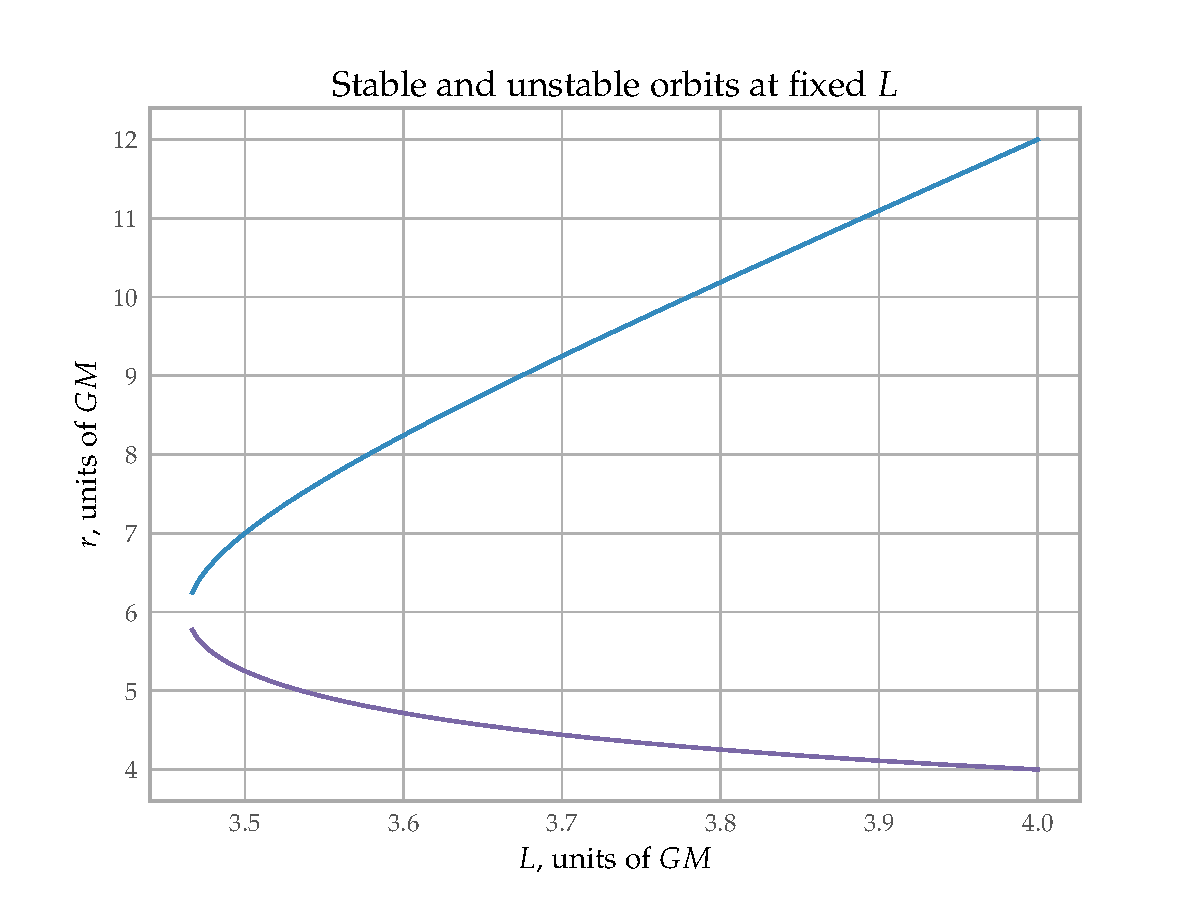
\includegraphics[width=\textwidth]{figures/fixed_L_orbits.pdf}
\caption{Allowed orbits at fixed \(L\). The unstable (lower) branch approaches \(r = 3GM\) asymptotically, the stable (upper) branch allows for arbitrarily large radii.}
\label{fig:fixed_L_orbits.pdf}
\end{figure}
  

For \(l _{\text{min}}\) we have \(r _{\text{min}} = 6 GM\).
This is called the ISCO: \emph{innermost stable circular orbit}: it is \(3\) times the Schwazschild radius \(2GM\).

\subsubsection{Orbital precession}

Now, we consider elliptical orbits.

The idea is: the angle between two consecutive perihelions is \(2\pi + \delta \varphi _{\text{precession}}\).

In order to find the orbits, we want a relation between different coordinates during the orbit: we will use the equations 
%
\begin{subequations}
\begin{align}
  l &= r^2 \dv[]{\varphi }{\tau }  \\
  \frac{1}{2}\qty(\dv{r}{\tau })^2 - \frac{GM}{r} + \frac{l^2}{2r^2} - \frac{GMl^2}{r^3} &= E 
\,,
\end{align}
\end{subequations}
%
so \(\dv{}{\tau } = \frac{l}{r^2} \dv{}{\varphi }\). Then: 
%
\begin{align}
  \frac{l^2}{2 r^2} \qty(\dv{r}{\varphi })^2 - \frac{GM}{r} + \frac{l^2}{2r^2} - \frac{GMl^2}{r^3} = E
\,,
\end{align}
%
and it is convenient to solve for \(u = r^{-1}\): we get 
%
\begin{align}
  \dv[]{r}{\varphi } = - \frac{1}{u^2} \dv{u }{\varphi }
\,,
\end{align}
%
so 
%
\begin{subequations}
\begin{align}
  \frac{l^2}{2} u^{4} \frac{1}{ u^{4 }} \qty(\dv{u}{\varphi })^2 - GMu + \frac{l^2u^2}{2} - GMl^2u^3 &= E \\
  \frac{1}{2}\qty(\dv{u}{\varphi })^2 - \frac{GM}{l} u + \frac{u^2}{2} - GMu^3 &= \frac{E}{l^2}
\,,
\end{align}
\end{subequations}
%
and we want to remove \(E\) so we differentiate with respect to \(\varphi \): 
%
\begin{align}
  \dv{u }{\varphi } \dv[2]{u}{\varphi } - \frac{GM}{l^2} \dv{u}{\varphi } + u \dv[]{u}{\varphi } - 3GM u^2 \dv{u}{\varphi } = 0
\,,
\end{align}
%
and the orbit is monotonic so \(\dv{u}{\varphi } \neq 0\): 
%
\begin{align}
  \dv[2]{u}{\varphi } + u = \frac{GM}{l^2} + 3GMu^2
\,,
\end{align}
%
where the term from \(GR\) is precisely \(3GMu^2\), the rest is fully Newtonian.

This can be solved exactly with respect to complicated elliptic function, but we do it in a simpler way: a nearly circular orbit: \(u = u_c (1+w(\varphi ))\), where \(w \ll 1\).

To the order \(w^{0}\): \(u_c = \frac{GM}{l^2} + 3GM u_c^{2}\), since it is a circular orbit (\(u_c\) is a constant!)

To first order in \(w\), instead, we get: 
%
\begin{align}
  u_c \dv[2]{w}{\varphi } + u_c(1+w) = \frac{GM}{l^2} + 3GMu_c^2 (1+2w)
\,,
\end{align}
%
since \(w \ll 1\). But the terms without \(w\) simplify: they satisfy the zeroth order equation. So, we are left with 
%
\begin{align}
  \dv[2]{w}{\varphi }  = (6GMu_c-1) w
\,,
\end{align}
%
which is in the form \(\ddot{w} + \omega^2 w =0\), since \(u_c < 1/(6GM)\). If we look at unstable orbits with radii smaller than \(6GM\), then this is exponentially diverging.

\end{document}